\documentclass{elegantbook}
\usepackage[square,numbers,sort&compress]{natbib}
\newcommand{\upcite}[1]{\textsuperscript{\textsuperscript{\cite{#1}}}}
\usepackage{multirow}
\usepackage{color}
\usepackage{tikz}
\usepackage{algorithm}
\usepackage{algorithmicx}
\usepackage{algpseudocode}
\renewcommand{\algorithmicrequire}{\textbf{Input: }}
\renewcommand{\algorithmicensure}{\textbf{Output: }}
\usetikzlibrary{shapes.geometric, arrows}
\tikzstyle{startstop} = [rectangle, rounded corners, minimum width = 2cm, minimum height=1cm,text centered, draw = black, fill = red!40]
\tikzstyle{acti} = [rectangle, trapezium left angle=70, trapezium right angle=110, minimum width=5cm, minimum height=0.5cm, text centered, draw=black, fill = blue!40]
\tikzstyle{pool} = [rectangle, trapezium left angle=70, trapezium right angle=110, minimum width=2cm, minimum height=0.5cm, text centered, draw=black, fill = purple!40]
\tikzstyle{process} = [rectangle, minimum width=3cm, minimum height=1cm, text centered, draw=black, fill = green!50]
\tikzstyle{conv} = [rectangle, minimum width=3cm, minimum height=1cm, text centered, draw=black, fill = magenta!50]
\tikzstyle{loss} = [rectangle, rounded corners, minimum width = 2cm, minimum height=1cm,text centered, draw = black, fill = yellow!40]
\tikzstyle{arrow} = [->,>=stealth]

% title info
\title{Deep Learning}
\subtitle{Sentence-level Sentiment Classification with RNN}
% bio info
\author{Yantian Luo}
\institute{Electronic Engineering}
\version{2018310742}
\date{\today}
\logo{logo.png}
\cover{cover.jpg}

\begin{document}

\maketitle
\tableofcontents
\mainmatter
\hypersetup{pageanchor=true}
% add preface chapter here if needed
\chapter{Introduction}
In this homework, we focus on fine-grained sentence-level sentiment classification problem. 

We use Stanford Sentiment Treebank (SST) dataset for experiments. This dataset contains 11,855 sentences, and has been splitted into the training / validation / test parts, containing 8,544 / 1,101 / 2,210 sentences respectively. Each sentence is categorized into one type of 5 sentiments. To preprocess the dataset, we use torchtext package. Before training the model, we need to tokenize words, building vocabulary, construct word embedding and intialize data iterator. torchtext has good wrappers for these operations and we can directly use dataloader in a similar way as before.

\chapter{Algorithm Design}
In this homework, we need to complete the forward process of RNNCell, GRUCell and LSTMCell using PyTorch. Considering these three cells have a common forward API: def forward(self, input, state). We can design the following algorithms.

\section{RNNCell}
We can use Algorithm \ref{alg:rnncell} to complete the forward process of RNNCell.

\begin{algorithm}[H]
	\caption{\label{alg:rnncell}the forward algorithm of RNNCell}
	\begin{algorithmic}[1]
		\Require input: $x$, hidden state: $s=[h, h]$(where $h$ is hidden state vector)
		\Ensure new state: $s'$
		\State $h' = \tanh( W_{ih}x + b_{ih}  +  W_{hh} h + b_{hh})$
		\State \Return $s'=[h', h']$
	\end{algorithmic}
\end{algorithm}


\section{GRUCell}
We can use Algorithm \ref{alg:grucell} to complete the forward process of GRUCell.

\begin{algorithm}[H]
	\caption{\label{alg:grucell}the forward algorithm of GRUCell}
	\begin{algorithmic}[1]
		\Require input: $x$, hidden state: $s=[h, h]$(where $h$ is hidden state vector)
		\Ensure new state: $s'$
		\State $r = \sigma(W_{ir} x + b_{ir} + W_{hr} h + b_{hr})$
		\State $z = \sigma(W_{iz} x + b_{iz} + W_{hz} h + b_{hz})$
		\State $n = \tanh(W_{in} x + b_{in} + r * (W_{hn} h + b_{hn}))$
		\State $h' = (1 - z) * n + z * h$
		\State \Return $s'=[h', h']$
	\end{algorithmic}
\end{algorithm}

\section{LSTMCell}
We can use Algorithm \ref{alg:lstmcell} to complete the forward process of LSTMCell.

\begin{algorithm}[H]
	\caption{\label{alg:lstmcell}the forward algorithm of LSTMCell}
	\begin{algorithmic}[1]
		\Require input: $x$, hidden state: $s=[h, h]$(where $h$ is hidden state vector)
		\Ensure new state: $s'$
		\State $r = \sigma(W_{ir} x + b_{ir} + W_{hr} h + b_{hr})$
		\State $z = \sigma(W_{iz} x + b_{iz} + W_{hz} h + b_{hz})$
		\State $n = \tanh(W_{in} x + b_{in} + r * (W_{hn} h + b_{hn}))$
		\State $h' = (1 - z) * n + z * h$
		\State \Return $s'=[h', h']$
	\end{algorithmic}
\end{algorithm}

\chapter{Results}
\section{Plot the loss value and accuracy value of one-layer RNN with 3 rnncells against to every epoch during training}
In this section, we use $lr=0.01, epochs=5$ with 3 rnncells to complete the experiments, and the loss value and accuracy value curves are as follow.
\subsection{RNNCell}
\begin{figure}[!h]
	\centering
	\begin{minipage}[t]{0.48\textwidth}
		\centering
		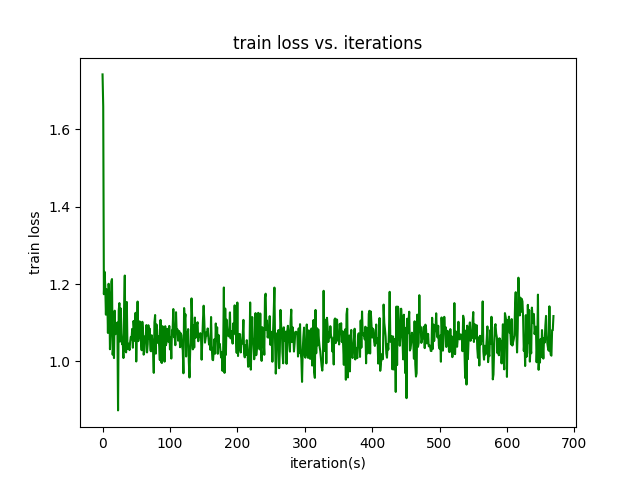
\includegraphics[width=\textwidth]{../codes/trainlossrnncell}
	\end{minipage}
	\begin{minipage}[t]{0.48\textwidth}
		\centering
		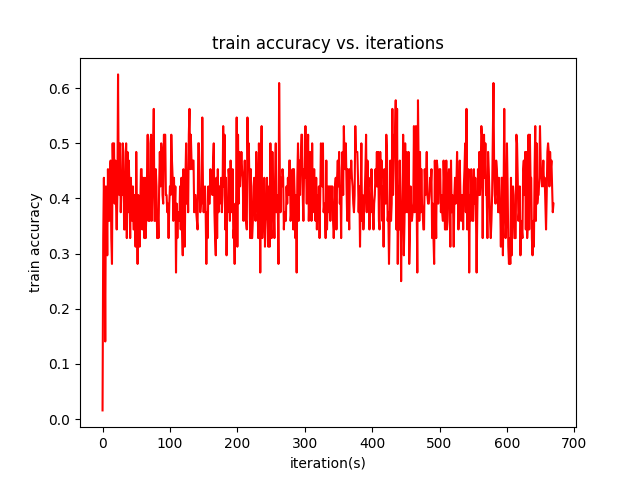
\includegraphics[width=\textwidth]{../codes/trainaccrnncell}
	\end{minipage}
	\caption{\label{trainres11}train loss curve and train accuracy curve using RNNCell against to every iteration}
\end{figure}

%\begin{figure}[!h]
%	\centering
%	\begin{minipage}[t]{0.48\textwidth}
%		\centering
%		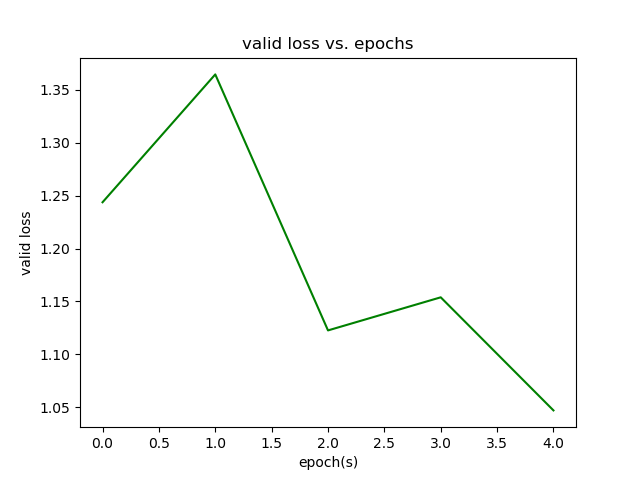
\includegraphics[width=\textwidth]{../codes/validlossrnncell}
%	\end{minipage}
%	\begin{minipage}[t]{0.48\textwidth}
%		\centering
%		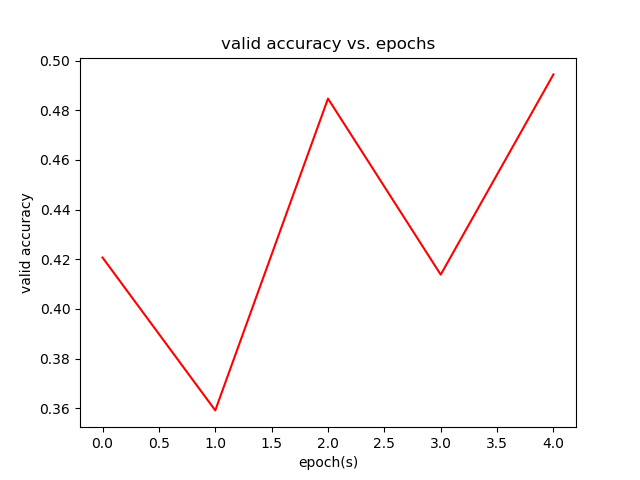
\includegraphics[width=\textwidth]{../codes/validaccrnncell}
%	\end{minipage}
%	\caption{\label{valres11}valid loss curve and valid accuracy curve using RNNCell against to every epoch}
%\end{figure}

\subsection{GRUCell}
\begin{figure}[!h]
	\centering
	\begin{minipage}[t]{0.48\textwidth}
		\centering
		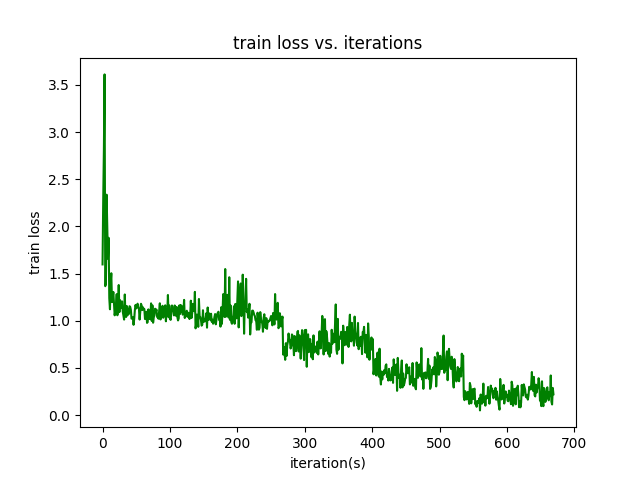
\includegraphics[width=\textwidth]{../codes/trainlossgrucell}
	\end{minipage}
	\begin{minipage}[t]{0.48\textwidth}
		\centering
		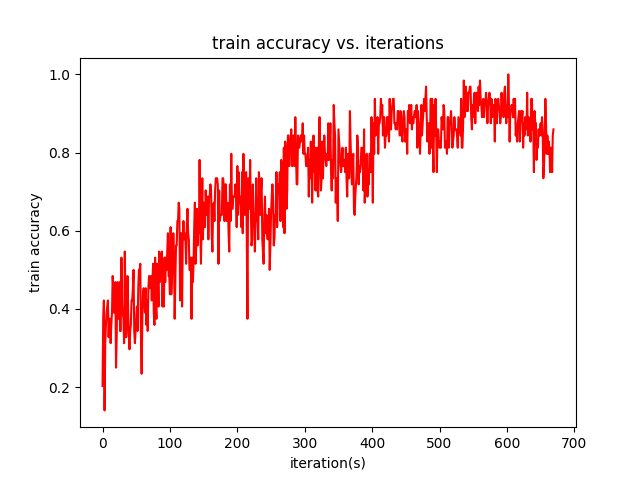
\includegraphics[width=\textwidth]{../codes/trainaccgrucell}
	\end{minipage}
	\caption{\label{trainres12}train loss curve and train accuracy curve using GRUCell against to every iteration}
\end{figure}

%\begin{figure}[!h]
%	\centering
%	\begin{minipage}[t]{0.48\textwidth}
%		\centering
%		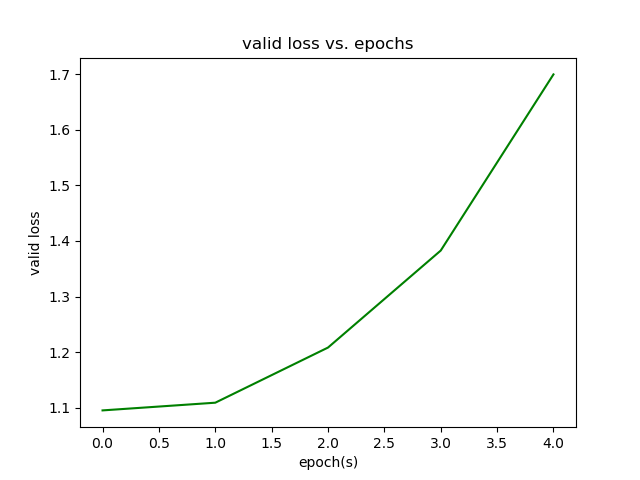
\includegraphics[width=\textwidth]{../codes/validlossgrucell}
%	\end{minipage}
%	\begin{minipage}[t]{0.48\textwidth}
%		\centering
%		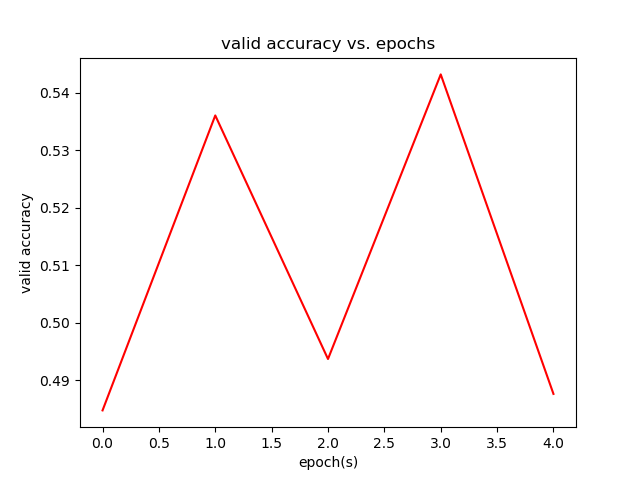
\includegraphics[width=\textwidth]{../codes/validaccgrucell}
%	\end{minipage}
%	\caption{\label{valres12}valid loss curve and valid accuracy curve using GRUCell against to every epoch}
%\end{figure}

\subsection{LSTMCell}
\begin{figure}[!h]
	\centering
	\begin{minipage}[t]{0.48\textwidth}
		\centering
		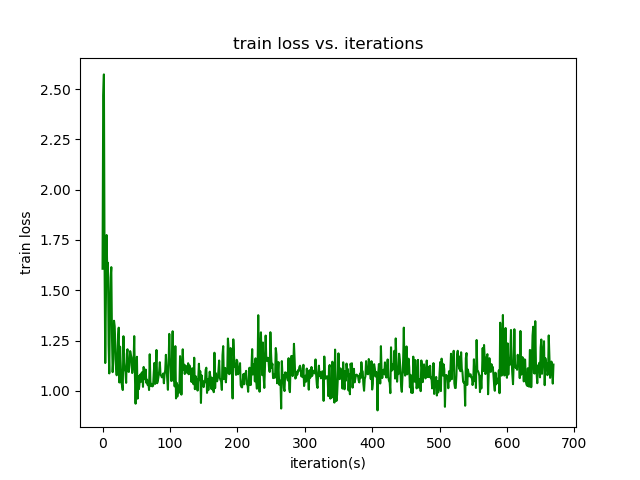
\includegraphics[width=\textwidth]{../codes/trainlosslstmcell}
	\end{minipage}
	\begin{minipage}[t]{0.48\textwidth}
		\centering
		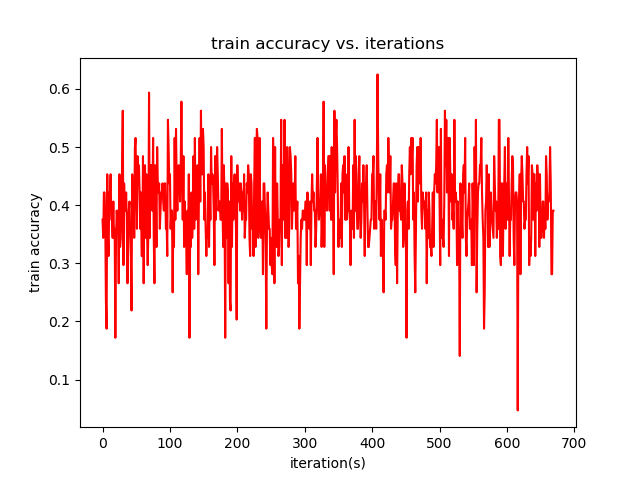
\includegraphics[width=\textwidth]{../codes/trainacclstmcell}
	\end{minipage}
	\caption{\label{trainres13}train loss curve and train accuracy curve using LSTMCell against to every iteration}
\end{figure}

%\begin{figure}[!h]
%	\centering
%	\begin{minipage}[t]{0.48\textwidth}
%		\centering
%		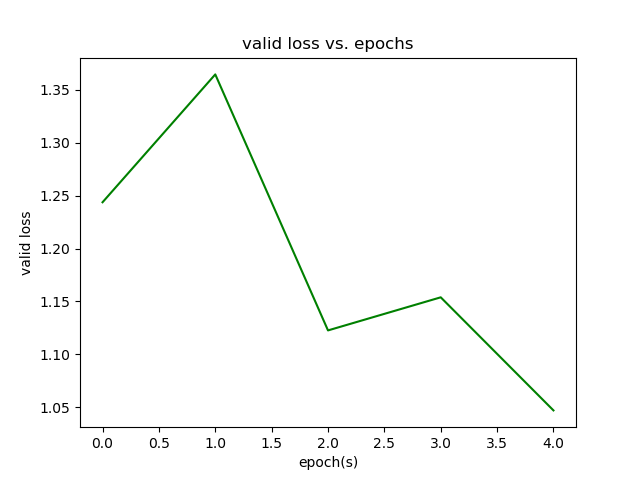
\includegraphics[width=\textwidth]{../codes/validlossrnncell}
%	\end{minipage}
%	\begin{minipage}[t]{0.48\textwidth}
%		\centering
%		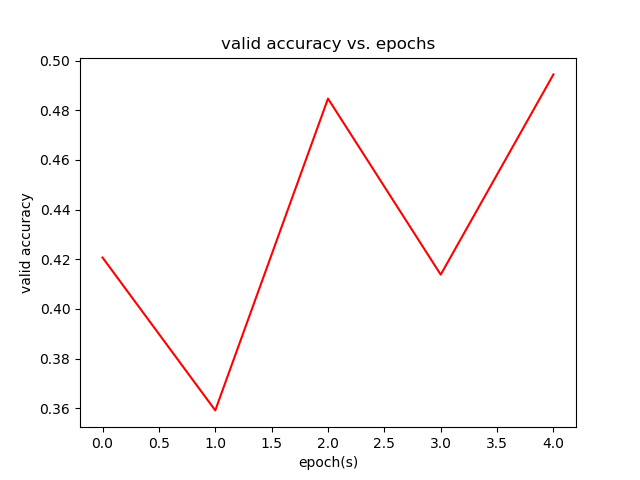
\includegraphics[width=\textwidth]{../codes/validaccrnncell}
%	\end{minipage}
%	\caption{\label{valres11}valid loss curve and valid accuracy curve using RNNCell against to every epoch}
%\end{figure}

\section{Compare and analyze the performance of the 3 rnncells}
We sum up the test results of 3 rnncells and list the results in Table \ref{res1}. From the table and the Figure in last section, we can find that:
\begin{itemize}
	\item Using RNNCell, the training speed is very fast but the test accuracy is not well;
	\item Using GRUCell, the training speed is also fast, and the test accuracy is better than RNNCell;
	\item Using LSTMCell, the training speed is very slow, and the test accuracy and test loss is better than RNNCell.
\end{itemize}

Therefore, we can find in this work, GRUCell is better than the other two rnncells.

\begin{table}[!h]
	\centering\caption{\label{res1}The comparison results of 3 rnncells}
	\begin{tabular}{|c|c|c|}
		\hline
		Cell Type & Test Accuracy & Test Loss \\
		\hline
		RNNCell & 0.5350 & 1.0595 \\
		\hline
		GRUCell & 0.5825 & 1.2509 \\
		\hline
		LSTMCell & 0.5765 & 1.0741 \\
		\hline
	\end{tabular}
\end{table}

\section{Using 100 dimensional embedding vector}
In this section, we use 100 dimensional embedding vector and GRUCell to do the experiment. We also plot the train loss curve and train accuracy curve against to every iteration in Figure \ref{trainres22}. The best test accuracy is 0.5945 and the best test loss is 1.2753. We can find that the test accuracy is a little better than before and the train speed is a litter fast because the dimension is a smaller than before.

\begin{figure}[!h]
	\centering
	\begin{minipage}[t]{0.48\textwidth}
		\centering
		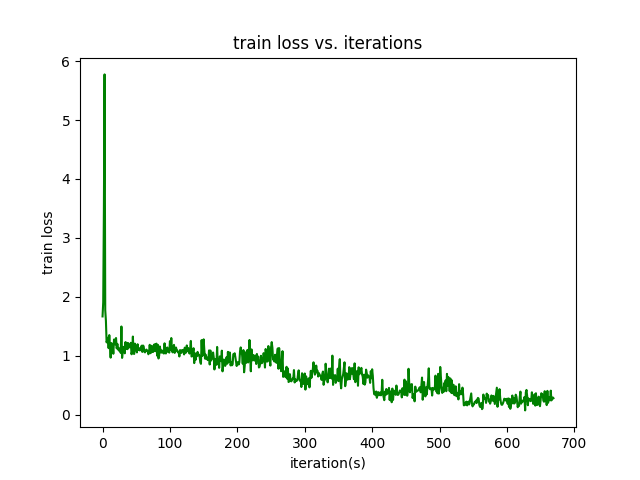
\includegraphics[width=\textwidth]{../codes/trainlossgrucell2}
	\end{minipage}
	\begin{minipage}[t]{0.48\textwidth}
		\centering
		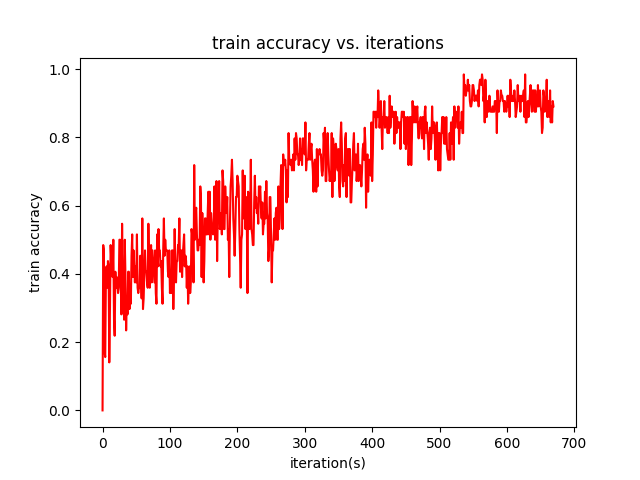
\includegraphics[width=\textwidth]{../codes/trainaccgrucell2}
	\end{minipage}
	\caption{\label{trainres22}train loss curve and train accuracy curve using 100 dimensional embedding vector against to every iteration}
\end{figure}

\section{Initialize embedding vectors without normal distribution}
In this section, we try to set $unk\_init=None$ to do the experiment that initialize embedding vectors without normal distribution. We also plot the train loss curve and train accuracy curve against to every iteration in Figure \ref{trainres32}. The best test accuracy is 0.6466 and the best test loss is 0.9108. We can find that the test accuracy and the test loss is much better than before.

\begin{figure}[!h]
	\centering
	\begin{minipage}[t]{0.48\textwidth}
		\centering
		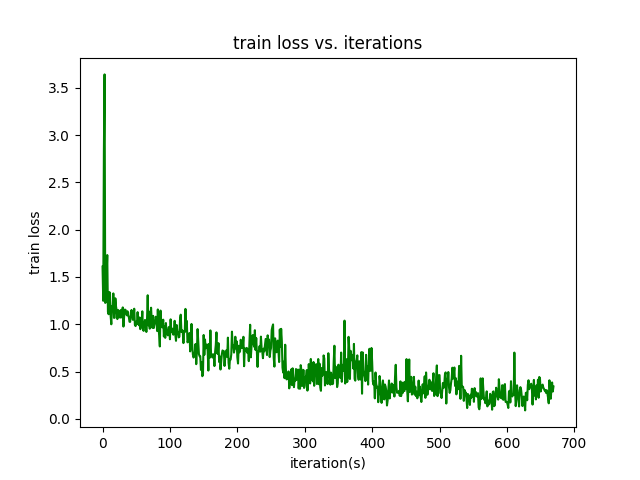
\includegraphics[width=\textwidth]{../codes/trainlossgrucell3}
	\end{minipage}
	\begin{minipage}[t]{0.48\textwidth}
		\centering
		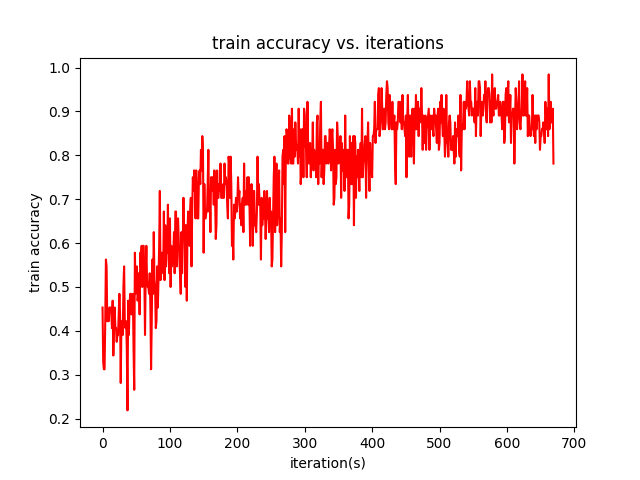
\includegraphics[width=\textwidth]{../codes/trainaccgrucell3}
	\end{minipage}
	\caption{\label{trainres32}train loss curve and train accuracy curve using 300 dimensional embedding vector and GRUCell without normal distribution against to every iteration}
\end{figure}

\end{document}